\documentclass[10pt]{article}
\usepackage[polish]{babel}
\usepackage[utf8]{inputenc}
\usepackage[T1]{fontenc}
\usepackage{graphicx}
\usepackage[export]{adjustbox}
\graphicspath{ {./images/} }
\usepackage{amsmath}
\usepackage{amsfonts}
\usepackage{amssymb}
\usepackage[version=4]{mhchem}
\usepackage{stmaryrd}

\title{Zestaw 3. }

\author{}
\date{}


\begin{document}
\maketitle
\begin{center}
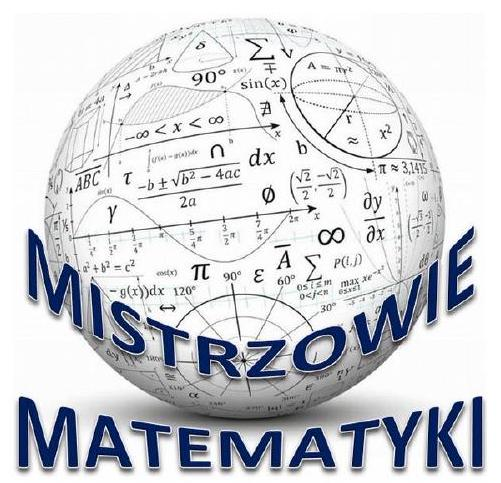
\includegraphics[max width=\textwidth]{2024_11_21_707bbc5bde3efcc74a79g-1(1)}
\end{center}

\section*{GIMNAZJUM}
\begin{enumerate}
  \item Liczbę 5797 rozłóż na sumę dwóch składników tak, aby jeden ze składników miał na końcu zero i aby po skreśleniu tego zera otrzymać drugi składnik tej sumy.
  \item Rozwiąż układ równań:
\end{enumerate}

\[
\left\{\begin{array}{l}
\frac{15}{x}-\frac{7}{y}=9 \\
\frac{4}{x}+\frac{9}{y}=35
\end{array}\right.
\]

\begin{enumerate}
  \setcounter{enumi}{2}
  \item W trójkącie prostokątnym środkowa poprowadzona z wierzchołka kąta prostego jest równa 10 i dzieli kąt prosty w stosunku \(1: 2\). Oblicz pole trójkąta.
\end{enumerate}

\section*{LICEUM}
\begin{enumerate}
  \item Dany jest trójkąt równoboczny \(A B C\) o boku 1 . Dla punktu \(X\) wewnątrz tego trójkąta przez \(p_{X}\) oznaczamy sumę pól trójkątów \(X A C_{X}, X B A_{X}\) oraz \(X C B_{X}\), gdzie \(A_{X}, B_{X}, C_{X}\) są rzutami prostokątnymi punktu \(X\) odpowiednio na boki \(B C, C A, A B\) (trójkąty zaznaczone na rysunku na szaro).\\
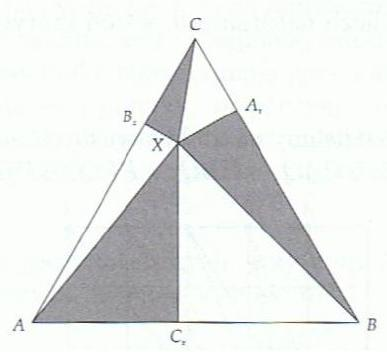
\includegraphics[max width=\textwidth, center]{2024_11_21_707bbc5bde3efcc74a79g-1}
\end{enumerate}

Znaleźć zbiór wszystkich możliwych wartości wyrażenia \(p_{K}-p_{L}\) dla punktów \(K, L\) z wnętrza trójkąta \(A B C\).\\
2. W trójkąt ostrokątny \(A B C\) o polu \(S\) wpisano kwadrat \(K L M N\) o polu \(P\) w taki sposób, że punkty \(K\) i \(L\) leżą na boku \(A B\), a punkty \(M\) i \(N\) leżą odpowiednio na bokach \(B C\) i \(C A\). Oblicz sumę długości boku \(A B\) i wysokości trójkąta \(A B C\) poprowadzonej z wierzchołka \(C\).\\
3. Pewna grupa liczy \(2 n+1\) osób. Każdy człowiek w tej grupie ma dokładnie \(n\) znajomych i \(n\) nieznajomych. Udowodnij, że \(n\) jest liczbą parzystą.

Rozwiq̨zania należy oddać do piq̨tku 30 stycznia koordynatorowi konkursu panu Jarosławowi Szczepaniakowi (tak długo, jak długo uda się go zastać w szkole :) lub swojemu nauczycielowi matematyki.


\end{document}